% !TeX program = lualatex
% !TeX root = main.tex
\renewcommand*{\dictumwidth}{0.5\textwidth}
\setchapterpreamble[u]{%
	\dictum[Andreas Bogk%\footnotemark
]{``UNIX is user-friendly, it just chooses its friends.''}}
\chapter{Introduction}
\label{chap:introduction}
\bigskip
\textit{An introduction into the field of High Performance Computing and the aspects of ``Green IT'' are given in this chapter. There is also a description about the goals and the structure of this thesis.}
%\footnotetext{\url{http://chaosradio.ccc.de/cr40.html}}

\bigskip

\lettrine[lines=2, lhang=.1, lraise=.1]{O}{n} today's computer systems, %\todo{anderer ansatz}
the CPU (central processing unit or simply processor) is the component which generally consumes the most energy, besides the GPU (graphics processing unit). The range lies between several watts in idle with activated power management and up to 110\,W under load for a CPU\cite{ht4uCPU}, and between 20\,W and 320\,W for a GPU\cite{ht4uGPU}. This is reflecting in the thermal design power (TDP) representing the maximum amount of heat the cooling system must be able to dissipate. 

This is also reflecting in the amount of power the computer system consumes and therefore the costs it causes. Especially when thousands of nodes with such CPUs respectively GPUs are active in a data center or HPC cluster. HPC stands for \emph{high performance computing} and, as the name suggests, its goals are offering high performance computing systems.

Additionally to CPUs a cluster needs a potent \emph{communication network} with high bandwidths, low latencies and adaptive routing, and storage nodes for backups and user files.
%
%
%\section{High Performance Computing}
%A HPC cluster is the result of duplicating this one node from the above example a few hundred or thousand times, combining them with a potent \emph{communication network} and adding storage nodes for backup and user files.
Such systems are needed in research and industry, mostly for simulations.
Some popular usage examples are
%
\begin{multicols}{2}
\begin{itemize}
	\item crash simulations
	\item protein folding
	\item climate research
	\item animation\,/\,special effects
\end{itemize}
\end{multicols}
%
\noindent
\emph{Parallelization} is crucial to get high performance by an adequate power consumption. Assuming the implementation of the application is not the bottleneck (the limiting factor), and there is the possibility to run the program in parallel, the only two ways for faster processing---except upgrading to newer processor types (or switching to another platform)---are either a higher processor frequency or more processors.

\newpage
To compare frequency scaling with processing unit (PU) duplication, two more assumptions are needed: 
%
\begin{enumerate}
\item processing speed scales linear with the frequency $f$
\item $P \,\propto \,U^2 \cdot f$ and $U \propto f$
\end{enumerate}
%
Now a small calculation shows what happens to the power consumption $P$ by rising the frequency and voltage $U$, or adding more PUs:
%
\begin{description}
\item[frequency scaling] $P_1$ is the consumption at normal speed. Doubling $f$ means $P_2 = (a \cdot U)^2 \cdot 2 f = 2 \cdot a^2 \cdot P_1$, whereas $a > 1$.
\item[duplicate processing unit] By doubling the processing unit, processing speed doubles too, at double power consumption: $P_2 = 2 \cdot P_1$
\end{description}
%
These are rough assumptions, but are legit for multi-core processors. But it is contra productive to produce processors with many cores at low frequency, because not all programs are (good) multi-threaded and would suffer from poor single-thread performance. Another reason is simply the limited space on a processor die, as more cores will need more space, together with a better inter-core network to unleash their full potential. The right balance between the number of cores and the actual processing speed per core is important.
%
\begin{wrapfigure}{R}{13em}
	\centering
	% !TeX program = lualatex
% !TeX root = ../../main.tex

\newcommand{\slice}[4]{
  \pgfmathparse{0.5*#1+0.5*#2}
  \let\midangle\pgfmathresult

  % slice
  \draw[thick,fill=gray!20] (0,0) -- (#1:1) arc (#1:#2:1) -- cycle;

  % outer label
  \node[label=\midangle:#4] at (\midangle:1) {};

  % inner label
  \pgfmathparse{min((#2-#1-10)/110*(-0.3),0)}
  \let\temp\pgfmathresult
  \pgfmathparse{max(\temp,-0.5) + 0.8}
  \let\innerpos\pgfmathresult
  \node at (\midangle:\innerpos) {#3};
}

\begin{tikzpicture}[scale=2]

\newcounter{a}
\newcounter{b}
\foreach \p/\t in {59/IT, 25/Cooling, 18/Power}
  {
    \setcounter{a}{\value{b}}
    \addtocounter{b}{\p}
    \slice{\thea/100*360}
          {\theb/100*360}
          {\p\%}{\t}
  }

\end{tikzpicture}
\newcommand*\Captiontext{typical energy consumption of a data center}
	\caption[\Captiontext]{\Captiontext\cite{cooling}}
	\label{fig:coolingpie}
\end{wrapfigure}
%

For multi-node systems (clusters) are many things not considered, for example the power consumption of the network and the other parts of a node (like mainboard, NIC, RAM or HDD). There is another reason against even higher frequency and therefore higher power consumption. The \emph{power density} %\,[$\frac{W}{cm²}$] 
 of the chip rises. There are limits how much heat a chip is able to bear before it dies. This is comparable to a glowing wire, before it melts. Modern processors have a power density of around 100\,$\frac{W}{cm²}$, which is nearly as much as a hot cooking plate.

In the end, the power is transformed into heat, which must be dissipated. Some fans and heat sinks on CPU and GPU are enough in a desktop computer. As place is limited in a building\,/\,room, cluster configurations are usually build of racks containing the dense packed nodes, offering the most hardware per amount of space. \emph{Cooling} is very important to guarantee the right environment for healthy equipment. As figure \ref{fig:coolingpie} shows, it is not unusual if cooling consumes more than 25\,\% of the power of the cluster, and another 15-25\,\% are consumed by the power supply (including uninterruptible power supply, general power conversions and efficiency of the power supply unit).

Popular ways of writing parallel programs are \emph{threads} for multi-core processors per single node and \emph{message passing} or \emph{virtual shared memory} for multiple nodes. Parallel programs have new ways of getting things wrong. Every line of code in a single-threaded program executes in order---besides compiler optimization or out-of-order-execution---whereas parallel programmes are hard to get in specific order. Access on shared variables or collective communication are indeterministic. Such \emph{race conditions} can even lead to a total halt, a \emph{deadlock}.

But the hard task is to get the result right and benefit from the multiple PUs---the application has to scale. \emph{Scalability} means the more cores calculate the faster the solution has to show up or the more data can be processed in the same amount of time.

The resulting performance boost by adding $N$ more processing units is called \emph{speedup}~$S$. It is ideally measured with the time $T_N$ using $N$ PUs against the time $T_1$ of a single-threaded program using the perfect algorithm for this problem---not against the parallel program running with one PU! How well the speedup is in regard to the used processing units is measured by the efficiency $E$\cite{ludwig}.
%
\begin{align*}
S &= \frac{T_{1}}{T_{N}}<N & E &= \frac{S}{N}<1
\end{align*}
%
There are two established laws concerning the ``prediction'' of scalability, whereas $P$ is the part of the program that is actually affected by the parallelization:
%
\begin{description}
\item[Amdahl's Law] $S = \frac{1}{(1-P) + \frac{P}{N}}$
\end{description}
%
Every program has parts that can not be split onto several PUs or that has to be done by every single PU, for example initialization or communication. This overhead is the reason why $E$ is really smaller than $1$.
The actual speedup now consists of the overhead $(1-P)$ and the parts getting faster processed $\frac{P}{N}$.

Gustafson takes another approach, because the part of a program causing the overhead is seldom executed often, mostly at the beginning and the end. The main purpose costing the most time of the program---the calculation---will be parallel, so $P$ is actually $1$ while calculating.
%
\begin{description}
\item[Gustafson's Law] $S = N - (1-P) \cdot (N - 1)$
\end{description}
%
%
\begin{figure}[ht]
	\centering
	%\hfill %
		\subfloat[Amdahl's law]{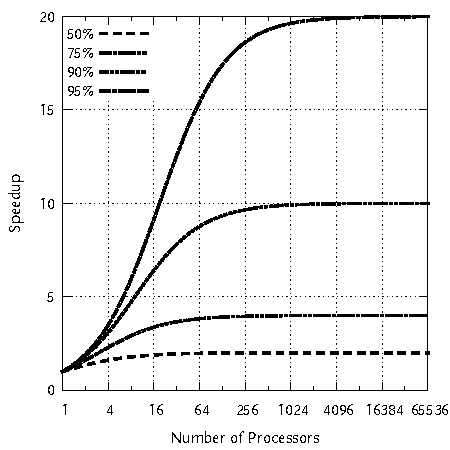
\includegraphics[scale=0.955]{pix/introduction/amdahl}}
	\hfill % alternativ auch \hspace{1cm} für genaue Angaben
		\subfloat[Gustafson's law]{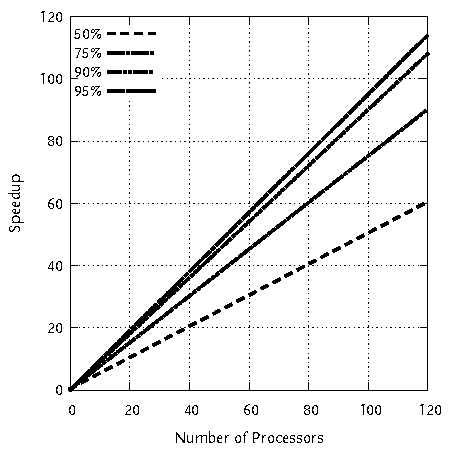
\includegraphics[scale=0.955]{pix/introduction/gustafson}}
	%\hfill %
	\caption{Amdahl's law and Gustafson's law}
	\label{fig:amdahl}
\end{figure}
%
%\newpage
%\noindent
As figure \ref{fig:amdahl} implicates, Amdahl's law predicts always a possible upper limit, whereas Gustafson's law does not. The reason is the difference opinion about the used \emph{problem size}. Problem size actually means the amount of data that has to be processed. Amdahl implicates a fixed problem size, so the calculating\,/\,communication ratio for every PU decreases when more PUs are used.

Gustafson predicts that the users will usually process more data (greater problem size) when they have more machines, mainly for getting more accurate results in the same amount of time.

Both laws are valid, as they target slightly different fields under different assumptions.

\superpar
The TOP500 project \cite{top500} aims to deliver statistics about the 500 most powerful general purpose HPC clusters in the world, and the technical development of those, because it helps manufacturers and (potential) users exchanging software and data, as well as establishing collaborations. The list is updated half-yearly (november and june) since 1993 and reflects the actual evolution in computing, as the aggregated performance of the list shows characteristics of Moore's law predicting a growth in performance by factor two every 18 months. Specific data about the computers are among others the number of cores, the power consumption, the theoretical performance ($R_{peak}$) and measured performance ($R_{max}$) in TFlops ($10^{12}$\,floating point operations per second, double precision). The measurement benchmark is LINPACK, which is basically a distributed solver for dense linear equation systems allowing architecture optimizations and variable problem sizes for achieving the best possible score per cluster.

%
\begin{table}[h!t]
	\caption{Abstract TOP500 List, November 2010}
	\label{tbl:top500}
	\centering
	\begin{tabular}{clcccc}
\hiderowcolors
		\toprule
			Rank	&Computer	&Cores		&$R_{max}$	&$R_{peak}$	&Power\\
					&			&			&[TFlops]	&[TFlops]	&[kW]\\
		\midrule
\showrowcolors
			1		&Tianhe-1A	&186\,368	&2566		&4701		&4040\\
			2		&Jaguar		&224\,162	&1759		&2331		&6951\\
			3		&Nebulae		&120\,640	&1271		&2984		&2580\\
			9		&Jugene		&294\,912	&826		&1003		&2268\\
		\bottomrule
	\end{tabular}
\end{table}
%
%\newpage

%\noindent
Table \ref{tbl:top500} shows four systems of the TOP500 list from november 2010. The first three have each more than one PFlops of measured performance, but also a power consumption of more than 2.5\,MW.
Jaguar drains nearly 7\,MW! For comparison, an average personal computer without monitor needs between 50 and 100\,W (at \approx 30\,GFlops $R_{max}$), a laptop with screen needs approximately 20\,W. 

%\noindent
An example breakdown of an actual cluster node can be seen in figure\,\ref{fig:powerconsumption}. Energy saving mechanics were not available---like in almost all clusters, because the main purpose of HPC is high performance, whereas general energy saving mechanics can lead to performance degradation. This picture should be applicable for many other cluster nodes and desktop machines---perhaps with lower CPU idle power consumption and one (or even more) additional GPGPU-cards (general purpose GPU).

%
\begin{figure}[H]
	\centering
	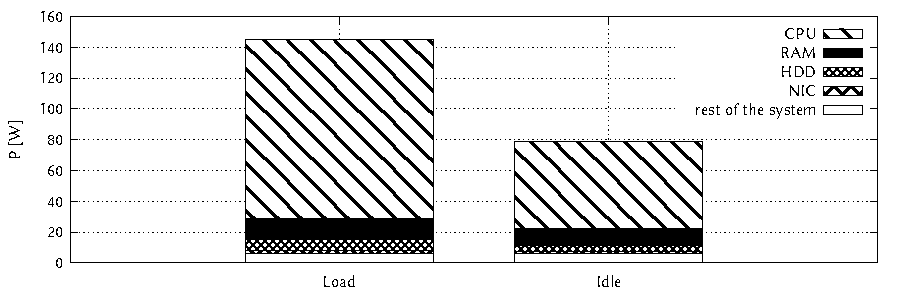
\includegraphics[width=\linewidth]{pix/systemconsumption/systemconsumption}
	\caption[System power consumption]{System power consumption\cite{minartz}}
	\label{fig:powerconsumption}
\end{figure}
%

%
%
\section{Green IT}
Like the name high performance computing implies, the goal in this area is performance. But energy efficiency gets more and more popular, as everyone seems to talk about CO$_2$ and the rising oil and energy prices. The Green500 project\cite{green500} takes the TOP500 list and reorders it considering the efficiency $\frac{MFlops}{W}$ based on $R_{max}$ and the power consumption. It is obvious by referring to table \ref{tbl:green500}, that high performance does not automatically imply energy efficiency, as the first ranked in the Green500 list delivers more than twice the energy efficiency than the first ranked in the TOP500, and more than six times than the second.
%
\begin{table}[h]
	\caption{Abstract Green500 List, November 2010}
	\label{tbl:green500}
	\centering
	\begin{tabular}{clrrr}
\hiderowcolors
		\toprule
			Rank	&Computer	&Efficiency	&Power	&TOP500 Rank\\
					&			&[MFlops/W]	&[kW]	&\\
		\midrule
\showrowcolors
			1		&NNSA/SC Blue Gene/Q Prototype	&1684.20	&39		&115\\
			11		&Tianhe-1A						&635.15		&4040		&1\\
			14		&Nebulae							&492.64		&2580		&3\\
			88		&Jaguar							&253.07		&6951		&2\\
		\bottomrule
	\end{tabular}
\end{table}
%

%\noindent
Application developers have to think about energy efficiency too, because bad program behaviour (e.\,g. polling) has impact on sleep time and the needed performance (e.\,g. algorithms) to finish a task.

But green IT means more than just energy efficiency. It is commercially relevant, as the consumer has direct advantages and a better feeling about ``helping the environment''. But even more important are the questions concerning the use of toxic materials or recyclability\,/\,reusability\,/\,refurbishability. Shamefully those topics are not well represented in mass-media, and many consumers do not even know where to dump their electronic waste. Those things are mainly handled and controlled by laws. A well-known example is ``RoHS'', which can be read on many stickers at electronic articles. RoHS stands for restriction of hazardous substances and describes limits of using toxic materials in products. Another example is the ``energy star standard'' which gives specifications about how much different devices (for example PCs or gaming consoles) are allowed to consume in active-, idle-, sleep- and standby-mode.\cite{greenIT}

%
%
\section{Goals and Structure of this Thesis}
HPC clusters need a large amount of power. Measuring this consumption for the whole cluster is very problematic, especially component measurement is only doable for few nodes, because special equipment is needed to record the consumption of a CPU or GPU. Such measurements are useful to find ways of saving energy or to predict the energy consumption after replacing components. In order to estimate at least the consumption of one of the main consumers---the CPU---a model based on its frequency and voltages will be presented and the needed data sources implemented.

\superpar
The rest of this thesis is structured as follows: 
chapter\,\ref{chap:model} deals with the calculation of the power consumption of a processor and how this can be approximated. Also some general strategies to reduce this consumption are listed.
Chapter\,\ref{chap:interfaces} lists some of the interfaces given by a modern Linux needed to get data like frequency and sleep time from a processor.
Some details about the projects that will be extended and used, as well as the actual implementation of the new features are described in chapter\,\ref{chap:implementation}.
Last but not least, chapter\,\ref{chap:evaluation} evaluates the processor model based on real world examples, and shows the functionality of the implementations.